\section{Multi-Layer Perceptron Classifier}
	    \pagestyle{mario}
	    \sectionauthor{M. Gini \& T. M. Hayden} %\printinunitsof{cm}\prntlen{\linewidth} this shows linewidth in cm

This section presents the multi-layer perceptron (MLP) classifier designed to classify the CIFAR-10 dataset. It is organized as follows: Section \ref{subsec:setup} introduces the basic software setup used to implement the MLP classifier. Section \ref{subsec:preProp} discusses the data preprocessing and augmentation. Section \ref{subsec:netStruct} analyzes the effect of different network structures on performance. Section \ref{subsec:optNet} analyzes what effect varying further hyperparameters like the error function or training algorithm have on the classification performance.

\subsection{Basic Software Setup}\label{subsec:setup}

The neural network toolbox from MATLAB is used to implement the MLP classifier.

\textcolor{red}{maybe picture of basic MLP network}
Since this is a classification problem, parts of the network structure are fixed. The last layer consists of 10 nodes and a in a "softmax" configuration. PICTURE of basic structure.
   	
As a default setup to analzye the effects of parameter variations, the following settings are used:

-stochastic gradient descent training method\\
-cross entropy error function\\
-etc etc\\

\subsection{Data Preprocessing and Augmentation}\label{subsec:preProp}
This subsection discusses the data preprocessing and augmentation.

a) on the selection of the inputs and outputs of the MLP
b) on the size of the training data 
 
\begin{itemize}
   	\item Data Preprocessing
  	
  	The input data is to the network consists of a 3072*1 array where the entries represent the raw pixel values. The pixel values are in the range [0,255]. To avoid any numerical issues and normalize the data, the data is divided by 255 to lie within the range [0,1]. Accordingly, the datatype is changed from the integer format to double. In a second step, the mean per pixel over the whole training set is subtracted. This centers the data.
  	
  	Optionally, we conduct experiments with whitened data. \textcolor{red}{here some plot to show effect of whitened data}
  	
  	\begin{figure}[h!]
  		\centering
  		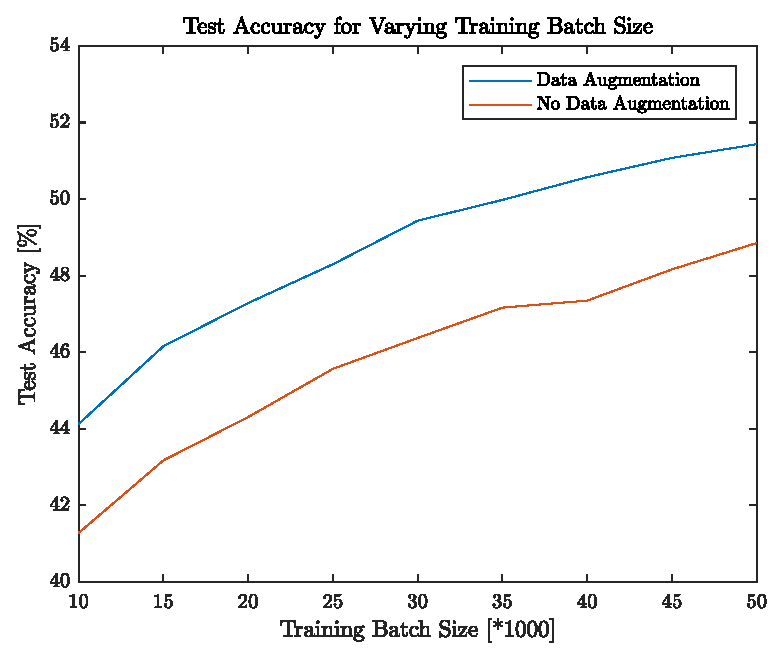
\includegraphics{images/dataAugmentation}
  		\caption{Hello Boy}
  		\label{fig:test1}
  	\end{figure}
  	
  	\begin{figure}[h!]
  		\centering	  		
  		\includegraphics{images/numberlayers}
  	  	\caption{Hello Boy2}
  	  	\label{fig:test2}
  	 \end{figure}
  	
  	Data preprocessing also includes the division of the complete dataset into appropriate training, validation and test data batches. The CIFAR-10 dataset consists of 60000 images, with 10000 specifically labeled for testing. For our performance analysis, we always use the provided test batch. The effect of varying training batch size can be seen below \textcolor{red}{here some plot of varying training size}
  	
   	\item Data augmentation
	    	
   	Experience shows that a larger training data set increases network performance. A basic and still successful data augmentation method is vertical mirroring. \textcolor{red}{here some plot of varying training size with mirrored data} When comparing with above, the increase in performance can clearly be seen.
   	
\end{itemize}
	    
\subsection{Optimization of Network Structure}\label{subsec:netStruct}
c)on the training of the MLP    
\begin{itemize}
   	\item Varying the number of neurons	
	\item Varying the number of layers	    	
\end{itemize}
	    
\subsection{Optimization of Network Hyperparameters}\label{subsec:optNet}
d) on the performance of the MLP with different objective functions and optimization methods
\begin{itemize}
   	\item Different learning rates
	    	
   	\item Different optimization methods
\end{itemize}
e)any other interesting observation that you think are pertinent (e.g. effect of learning rate on convergence speed).